\documentclass{sig-alternate}

% *** SPECIALIZED LIST PACKAGES ***
%
\usepackage{algorithmic}

\usepackage{array}

% *** PDF, URL AND HYPERLINK PACKAGES ***
%
\usepackage{url}

\begin{document}

% Copyright
\setcopyright{acmcopyright}
%\setcopyright{acmlicensed}
%\setcopyright{rightsretained}
%\setcopyright{usgov}
%\setcopyright{usgovmixed}
%\setcopyright{cagov}
%\setcopyright{cagovmixed}

%Conference
\conferenceinfo{GECCO '16}{Denver, CO, USA}
% --- End of Author Metadata ---

\title{Visualizing for success: making the user more efficient in
  interactive evolutionary algorithms}
%
% You need the command \numberofauthors to handle the 'placement
% and alignment' of the authors beneath the title.
%
% For aesthetic reasons, we recommend 'three authors at a time'
% i.e. three 'name/affiliation blocks' be placed beneath the title.
%
% NOTE: You are NOT restricted in how many 'rows' of
% "name/affiliations" may appear. We just ask that you restrict
% the number of 'columns' to three.
%
% Because of the available 'opening page real-estate'
% we ask you to refrain from putting more than six authors
% (two rows with three columns) beneath the article title.
% More than six makes the first-page appear very cluttered indeed.
%
% Use the \alignauthor commands to handle the names
% and affiliations for an 'aesthetic maximum' of six authors.
% Add names, affiliations, addresses for
% the seventh etc. author(s) as the argument for the
% \additionalauthors command.
% These 'additional authors' will be output/set for you
% without further effort on your part as the last section in
% the body of your article BEFORE References or any Appendices.

\numberofauthors{3} 
\author{
\alignauthor
Juan-J.~Merelo\titlenote{Corresponding author}\\
\affaddr{Dept. of Computer Architecture and Technology and CITIC}\\
\affaddr{University of Granada, Granada, Spain} \\
\email{jmerelo@ugr.es}
\alignauthor
Mario Garc\'ia-Valdez \\
\affaddr{Dept. of Graduate Studies}\\
\affaddr{ Instituto Tecnol\'ogico de Tijuana, Tijuana, Mexico}\\
\alignauthor
Carlos Cotta\\
\affaddr{Dept. LCC, ETSI Inform\'atica}\\
\affaddr{ Universidad de M\'alaga, M\'alaga, Spain}\\
}

\maketitle

\begin{abstract}

Using volunteer's browsers as a computing resource presents several
advantages, including cost, but it remains a challenge to fully harness the browser's
capabilities and to model the user's behavior so that those
capabilities can be leveraged optimally. One of the main challenges,
and heretofore not addressed, is how to first keep the user engaged in
the experiment so that his computation time is maximized, and second
and second how to present the information in such a way that the participation 
also becomes call to action, where volunteers can operate parts of the 
evolutionary algorithm itself thus becoming, even more, an integral part of the
experiment. This paper is not a presentation 
of results, but rather a call for comments to find out how to address
these problems in the most systematic way. 
%
% This sentence is not clear to me: 
%and second
%how to present the information in such a way that it can be a call to
%action that can, actually, help the evolutionary algorithm itself by
%doing any number of operations on it.
% operations on the algorithm? 
% like what operations? re-start the algorithm etc?
% Maybe something like:
% and second how to present the information in such a way that the participation 
% also becomes call to action, where volunteers can operate parts of the 
% evolutionary algorithm itself becoming an integral part of the
% experiment.
%done - JJ


\end{abstract}

\keywords{Volunteer computing, distributed computing, cloud computing,
visualization}


%---------------------------------------------------------------
\section{Introduction}

In volunteer computing systems, one of the objectives is to get the
user give as much time as possible to the experiment. Most of the
efforts nowadays include gamification, but these have the problem that
a competition has an implicit incentive to cheat to get ahead of your
competitors. 

In the case of systems such a NodIO \cite{2016arXiv160101607M}, which
is a minimal infrastructure to support pool-based distributed
evolutionary computing experiments, there is another issue with the
user. NodIO has been used for volunteer computing experiments by
embedding an island-based evolutionary algorithm inside a web page and
making them interchange information via the NodIO server, in a
spontaneous and eventually panmictic distributed evolutionary
algorithm. In the experiments we have carried out so far we have
realized that the way the user perceives the state of the algorithm
can make him or her act in several ways. For instance, reloading the
page, in which case a new population will be generated, with the best
individuals being sent to the pool adding to the diversity of that
pool. The user can also load the webpage in several browsers or
browser tabs so that it is adding more power and seeing how the
solution spreads from one to the other. In any case, we have noticed
that the user spontaneously is making it an {\em interactive}
algorithm \cite{takagi01interactive}, by applying {\em hypermutation} operators or even {\em
  distributing} themselves the population if their machine performance
allows them to do so. 

However, it will be impossible for the user to perceive what is
happening if the visualization does not convey that information in a
way that can be first understood by anyone without using any technical
term and second does not add too much overhead to the algorithm
itself. As far as we know, the problem of visualizing an evolutionary
algorithm so that the non-technical and spontaneous user can help it
find the solution faster has not been fully solved. We have made several
attempts that we will present in this paper, but this paper is
basically a request for comments during the workshop and later on so
that the scientific community understands the basis of this problem
and can also design their own solutions for it.  

That is why the rest of the paper will be devoted to a short state of
the art, an exposition of our efforts so far and finally instead of
conclusions several research questions that we hope are the bases for
a discussion of this issue.



%---------------------------------------------------------------
\section{State of the art}
\label{sec:soa}

As far as we have been able to find, there is no research devoted
exclusively to visualization to maximize involvement and interactivity
in volunteer computing experiments. From the very beginning,
BOINC@home included visualization of the results of the computation
\cite{anderson2006designing}, but it was only for informative
purposes, not a part of the system itself. 

There has been, however, a certain amount of research in interactive
evolutionary algorithms, e.g., \cite{takagi01interactive,parmee:human-centric2003,parmee08user-centric,badillo13usercentric}, 
where users perform all or some evolutionary
operations; in our case, since the
user has control of the browser, there is a limited amount of
interaction with it, namely, the fact that by reloading the webpage they
can apply a kind of hypermutation, killing the current population and
generating new individuals some of which will make their way to the
common pool via migration. In that sense, volunteer computing is also
a way of {\em human computation} \cite{quinn2011human}, a concept that
has also been applied to evolutionary algorithms \cite{972056, Nickerson2013}, in
this case extensively and with all operators. In general, these type
of human based evolutionary algorithms must be constrained to those in
which the problem representation can be understand by us; 
For example, some early approaches 
\cite{Daw86} relied on the visualization of solutions so that the user can 
pick his/her preferred ones. In a more general approach, \cite{takagi-jcis2000} 
considered the utilization of dimensionality-reduction techniques in order
to project the population of solutions to a more amenable space (a 2D plane)
on which the user can express his preferences. The work of Deb et al. in
multi-objective optimization \cite{DC07,DK07} was similarly aimed to direct 
the exploration toward particular regions of the Pareto front.
\cite{cheng2004interactive} mentions evolution of text messages and
applies it to evolution of colors, where users have to pick up two
colored blocks to perform crossover; this is later on extended to the
OneMax problem, comparing the performance of a human operator who does
not know the shape of the fitness function with that of an interactive
evolutionary algorithm where the user himself is the one that acts as
fitness evaluator.
However, the visualization performance or the latter evolutionary algorithm is
eschewed, so that the only hint
that the user has of how the algorithm is doing is the fitness itself
or, even, just a hint of how close the user is to his desired
value. This is the problem we have been trying to solve and we will
show our solutions below, before calling for others in the last part
of the paper. 

\section{Description of the system and some results}
\label{sec:res}

NodIO \cite{2016arXiv160101607M,DBLP:conf/gecco/GuervosG15} is a
web-services based system that allows to run distributed evolutionary
computing experiments, including volunteer computing systems, with a
low overhead. 

The common part of all algorithms is the server, that has been
published with a free license in GitHub, which includes several REST
(Representational state transfer)
routes, which are remote procedure calls using the HTTP (Hypertext
Transfer Protocol). In practice, that means that clients use a
standard and well known interface, HTTP, to communicate with it and
clients can be written in many different languages, including
JavaScript on the client  or Perl. 

The server receives individuals from the client using the {\tt PUT}
HTTP command. The individual received is stored in a cache that is
refreshed in sub-second intervals, currently set at 0.2 seconds, and
has a finite size equal to 32, although it can contain a few elements
more before the refreshing period finishes. The finite cache is used
for implementation but also algorithmic reasons; it needs to be finite
to limit the amount of memory used by the server, which could blow up
to a size too big for the server, but from the algorithmic point of
view, it is also  a good practice to keep only the latest solutions so
that the clients are sent one of them, instead of one of many created
during the whole experiment. 
The cache is renovated in a First
In, First Out fashion, which, from the point of view of the
evolutionary algorithm, contributes to the diversity of the stored
population, since it is renovated from time to time. In general, this way of using a stored population from
which some individuals are drawn is called a pool-based evolutionary
algorithm
\cite{pool:ga,bollini1999distributed,gong2015distributed,
  sofea:evopar2012,DBLP:journals/grid/ValdezTGVO15,garcia2014unreliable,LNCS86720702,
  DBLP:conf/3pgcic/GuervosMFEL12,sofea:naco}; this type of
asynchronous and persistent algorithm lends itself better for the
ephemeral and dynamic computing environment in which we are
working. 

The server receives the chromosome and its fitness and
 stores them returning to the client a random individual from the
cache and some more information, like the cache size at this
particular moment. This cache size information can be used by the
client for detecting when the current algorithm has found a solution,
or also for visualization purposes. A function for detecting when the
solution is found is used and, when that happens, the cache is emptied
and a variable that keeps track of the experiment number is
incremented. In principle, any of those indicators can be used by the
clients to check whether the experiment has finished or not. 

The clients run an island-based evolutionary algorithm for solving the
50-Trap problem programmed in JavaScript using a browser version of
the NodEO library \cite{DBLP:conf/gecco/GuervosVGES14,figshare:nodeo,nodeo2014}. It is a difficult combinatorial optimization and
deceptive problem which has been chosen mainly for the time and the
population size it needs to succeed. Deceptive problems are known for
the high diversity they need for finding the solution; this diversity
must be in the initial population or else maintained in the population
by using different mechanisms. However, the population of every client
has to be kept low to avoid overloading the volunteer computer;
currently it is 128 individuals, and other mechanisms will need a
level of analysis that is incompatible with the ephemeral nature of
the system. Every 100 generations, the client sends using HTTP PUT the
best chromosome to the server, receiving in return a random chromosome
from the cache and the cache size. If the client finds the solution,
it stops. If the client finds that cache size has decreased by a
certain number, it reloads the page, restarting the population all
over again, avoiding overlapping ``old'' results with the new
experiment.
 
\begin{figure}[!htb]
\centering

\includegraphics[width=0.99\linewidth]{tweet.png}
\caption{Tweet asking for help in the volunteer computing experiment,
  and also showing the amount of retweets and date. In most cases,
  tweets were in Spanish. The URL mentioned is active at the time of
  writing this paper. \label{fig:tweet}}
\end{figure}
%
In order to run the experiments, we announced it in social networks
via a tweet, WhatsApp message, Facebook post, Telegram message or, in
some occasions, LinkedIn. One of the announcements is shown in Figure
\ref{fig:tweet}. Volunteer computing cannot be understood without its
social part, since it needs a continuous inflow of new
users, but so far there is no relation to the algorithm itself or the
current situation. Using social networks to visualize the progress of
the algorithm is also an area that might be interesting to explore. 

\begin{figure*}[!htb]
\centering
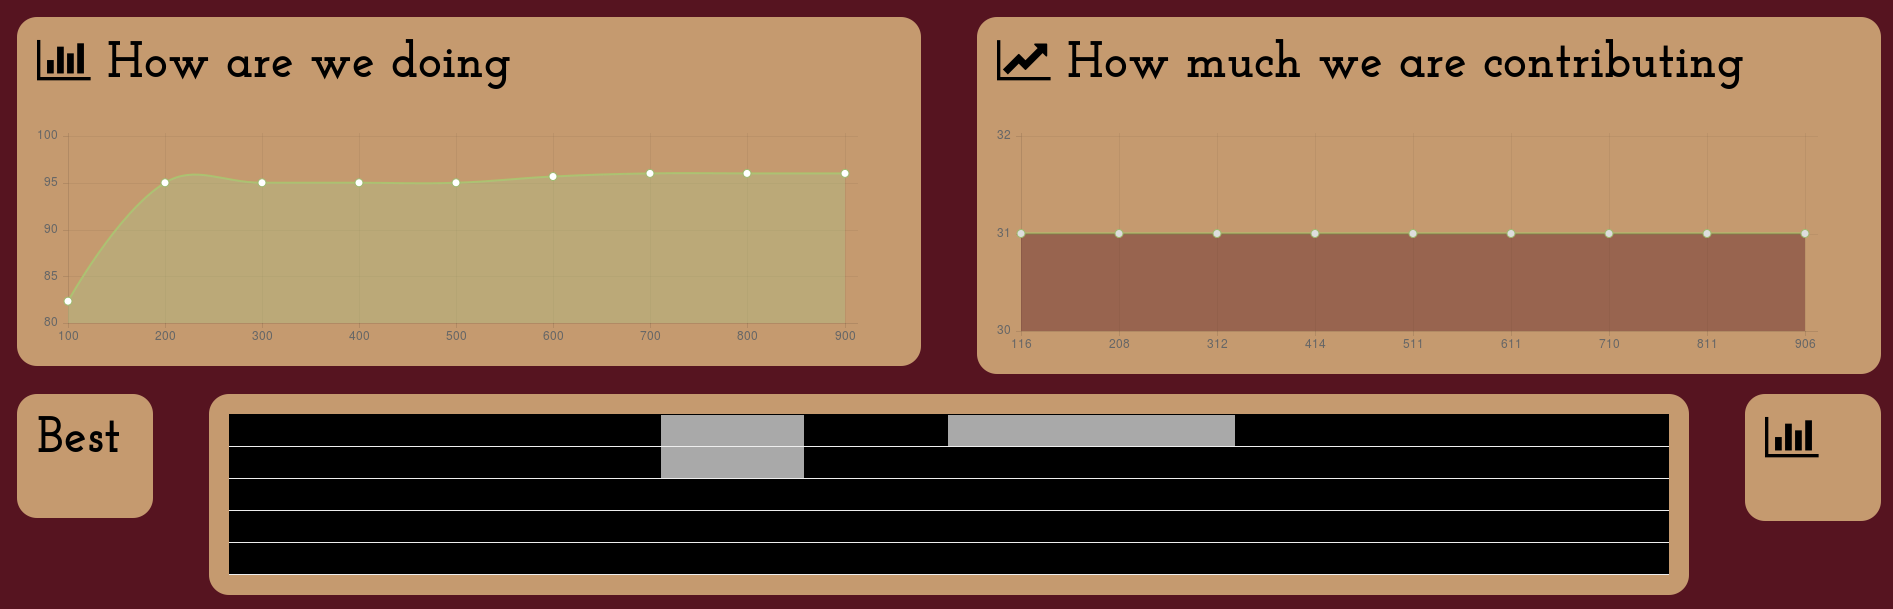
\includegraphics[width=0.95\linewidth]{all.png}
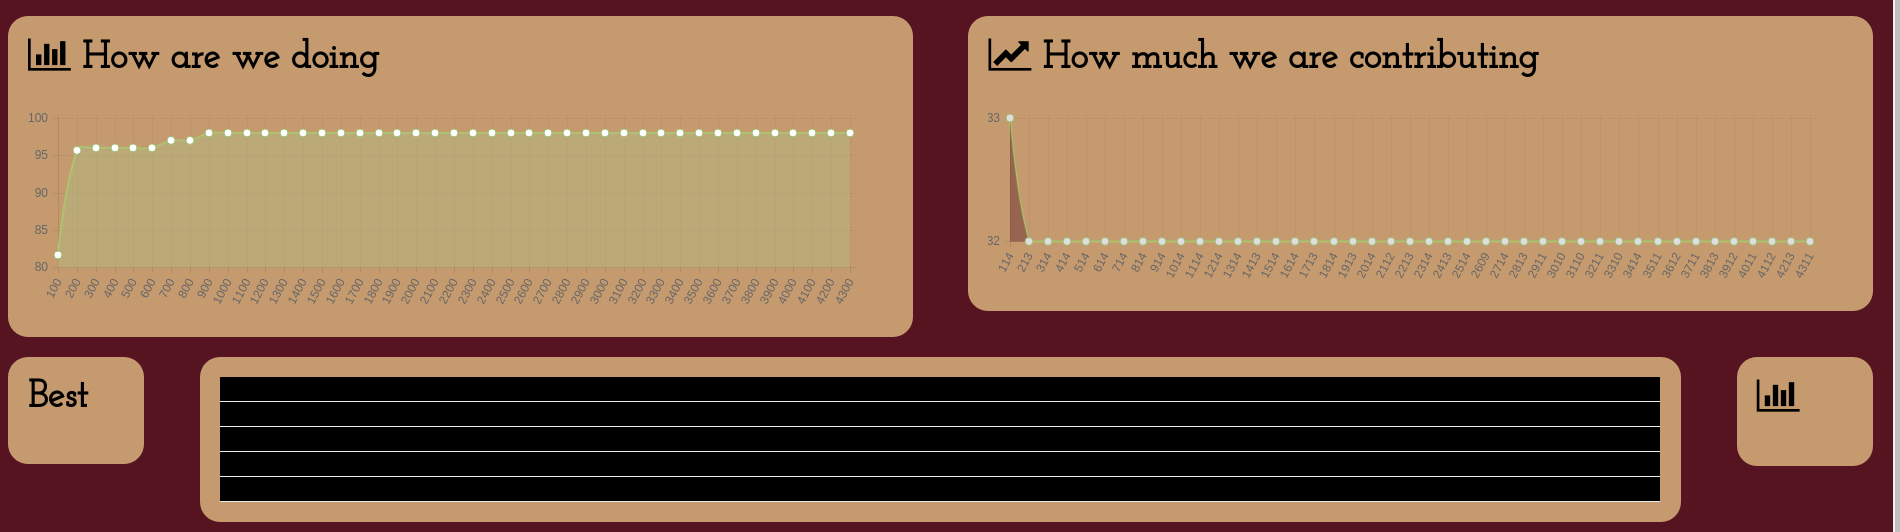
\includegraphics[width=0.95\linewidth]{finish.png}
\caption{The three panels showing the latest fitness, the cache size
  and the best chromosome using 4 shades from white to black to
  represent the number of ones in every block in the Trap
  problem at the top; at bottom, the finished algorithm showing 5
  black bars indicating that the 50 traps have been found. \label{fig:all}}
\end{figure*}
%
The client displays three panels, showing three different
visualizations of the evolutionary algorithm. Two of them have been
kept fixed for all experiments, and they are shown in Figure
\ref{fig:all}. The top panels show, to the right, the fitness in the
last 5000 generations at 100 generations interval. The bottom panel
shows a visualization of the best individual, using blocks that
represent the number of ones in 4-bit blocks with different colors
that represent their block fitness, from 0 (transparent) to 2
(black). 1 is the intermediate fitness, achieved with all 0s, and it
is represented by dark gray. 

From the point of view of the user, this is probably one of the best
indicators of the stagnation of the simulation. The most likely
situation is to have that panel stuck with all blocks in black except
one in gray, with the fitness stuck at 99. If that happens for a long
time, it is almost impossible for a single island to find the
solution, because it is stuck in a local minimum from which it is
impossible to get out with a single mutation; it needs a string of
favorable mutations, all of them having a lower fitness. So in
principle that situation could help the user to restart the simulation
in that case, but it is almost impossible for the user to forecast
when that will be happening and avoid it, either by restarting or by
starting it in other browser tabs. 

\begin{figure}[!htb]
\centering
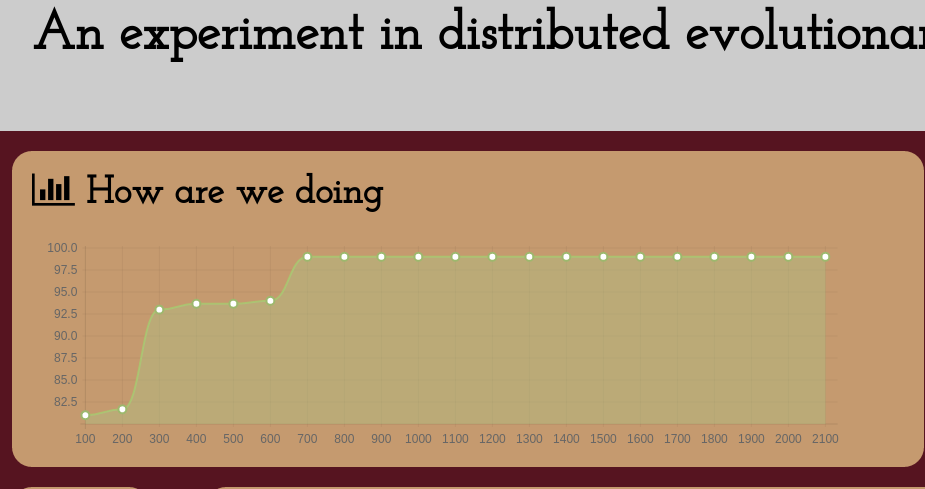
\includegraphics[width=0.95\linewidth]{fitness.png}
\caption{This panel, labeled with ``How are we doing'', shows
  the evolution in time of the fitness, it rotates to show only the
  last 5000 generations.  \label{fig:fitness}}
\end{figure}
%
This information might be redundant with that shown in the fitness
panel, shown in Figure \ref{fig:fitness}. However, it helps when you
have several windows, side by side. If the best chromosome is the same
in both, not only a single island is stuck, but the whole number of
islands contributing are. That happens usually when there is a single
island running for some time in that situation and all of a sudden
several other volunteers come in. As soon as they start to receive
random individuals from the cache, they are bound to get that {\em
  super} individual, which will eventually {\em invade} the
population, crashing global diversity. The best situation is when
several individuals arrive at short intervals, contributing diversity
but also individuals that are not so different; by the {\em
  intermediate disturbance hypothesis} \cite{jj:2008:PPSN} that
situation will boost the performance of the whole system. However, the
user in general will run a single tab, so they will not know that is
happening; this is a kind of information that we would need to convey
to the user by way of visualization. But that is why we use the third
panel. 

\begin{figure}[!htb]
\centering
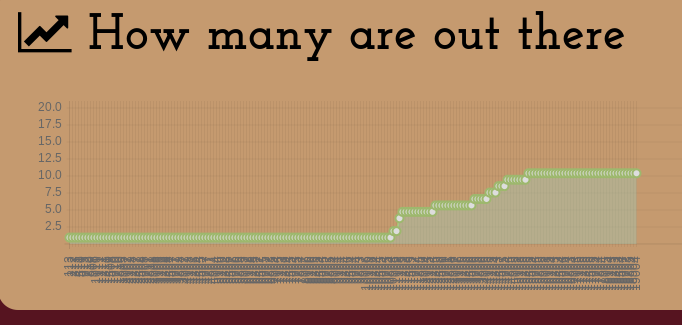
\includegraphics[width=0.95\linewidth]{howmany.png}
\caption{This panel, labeled with ``How many are out there'', shows
  the number of different IPs that are contributing to the simulation,
  accumulated since the beginning of the simulation run.  \label{fig:howmany}}
\end{figure}
% 
Initially we used as third panel the number of IPs that had
participated so far, shown in Figure \ref{fig:howmany}. This was
mainly for the benefit of us, not really the user; it was a way of
knowing the impact of some particular announcement and also to see how
many users were there at a particular time. However, the user could
gather no information either about his particular involvement or about
the progress of the simulation. Besides, it was the {\em total} number
of IPs from the beginning of the batch of experiments, it did not show
the instantaneous, or in the last minutes, number of participating
IPs. That is why we opted to change that visualization to a new one
that at least included some information on it. 

\begin{figure}[!htb]
\centering
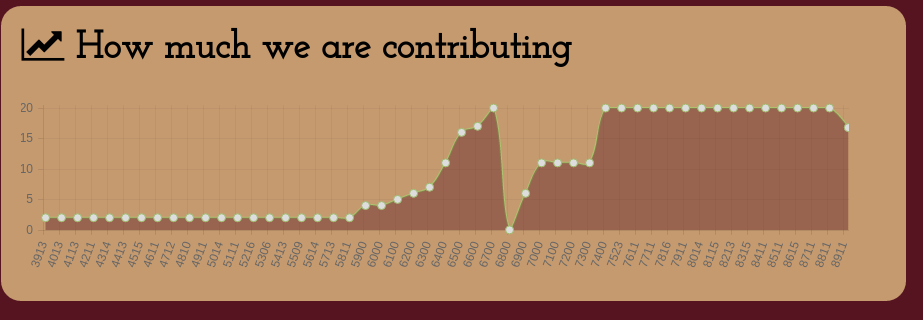
\includegraphics[width=0.95\linewidth]{contribution.png}
\caption{This panel, labeled with ``How much I am contributing'', in
  fact shows the cache size. Cache increases when new individuals are
  added to the pool; it stays the same if the users keep sending the
  same individuals. The graph shows the activity of the last 5000
  generations in a rotating fashion, eliminating the first as new ones
  arrive. In this case the cache has changed size since some other
  user has found the solution.   \label{fig:howmuch}}
\end{figure}
%
Figure \ref{fig:howmuch} was labelled {\em how much I am
  contributing}. That is not exactly what is shown in the graph, that
shows the cache size. However, if you combine this panel with the
other, and the fitness panel and the chromosome panel shows some
change, you will see if that change is incorporated to the cache if
that changes size. If the cache remains the same, no new individuals
are being generated and again you can have a perspective of the whole
experiment being stagnated in a single view; the user can then decide
to restart or also to create new populations. It is still a poor way
of conveying global information and it requires a certain amount of
information given to the user so that he or she can understand what is
going on.

In order to see whether this new panel was more effective from the
point of view of the user interaction than the previous one, we
measured the amount of {\em reboots}, that is, new initializations of
population by the user, either by restarting one window or starting
new ones. In order to measure this effectivity, we measuered the
amount of reboots per IP. When the first graph was used, the average
was 0.74; the second graph, depending on the batch of experiments,
registered averages over 1, 1.58 in a first batch, 1.16 in a second
batch, both carried out in the month of February and March, indicating
an average of more than 1 reboot per user. This might indicate that
showing more information to the user, specially about the global
progress of the experiment, encourages them to act on it, by using the
only tool they have: reloading the page, thus restarting the
experiment, or loading it in new pages. And that is also the reason
why we think that using innovative ways of visualization will
encourage them to interact even more with it, turning it into a truly
interactive experiment. 


%---------------------------------------------------------------
\section{What can be visualized and how it could help}
\label{sec:conclusion}

For the time being, the only possibility the user has is to start  or
restart new islands. However, this need not be the only way the user
can help the simulation. Even keeping the interface as simple as
possible, other possibilities could include:\begin{itemize}
\item {\em Killing} the best individual, thus immediately creating
  diversity by having the rest compete.
\item Increasing or decreasing the population size. A bigger
  population will have higher initial diversity.
\item Increasing or decreasing the mutation or crossover rate. For the time being,
  bitflip mutation is used on every new generated individual. Maybe it
  could be decreased to a lower percentage, or increase the number of
  bits flipped for every individual generated.
\end{itemize}

However, even if whatever the user does will contribute to diversity,
if it is done blindly will explore more than exploit and be thus a
waste of computational resources. That is why there are several
possible ways of showing progress and diversity, which is a predictor
for future progress:\begin{itemize}
\item Represent the convergence of the population towards a single
  individual by showing, using grayscale, the uniformity of values for
  all bits. This can be represented alongside the best one, or maybe
  instead of the best one.
\item Represent global diversity by having a measure of compression
  entropy plotted, instead or alongside the cache size.
\end{itemize}

This can be complemented by other visualization measures, such as \begin{itemize}
\item Use Twitter or a Telegram channel to represent the progress of
  the current experiment, or making calls when a new experiment has
  started to have an early infusion of diversity.
\item Represent the progress of the particular user against the rest
  of the users, showing the fitness of every one, for instance, or the
  time every one has spent represented by the number of PUTs that have
  been made. The fitness has the problem that, after certain time, all
  fitness would be the same. However, this can be seen as an indicator
  that the experiment has stagnated and thus a restart has to be made.
\item Keep past history and represent current experiment comparing its
  progress to the progress of previous ones.
\item Show global fitness alongside local fitness. Once again, global
  best fitness (as contained in the cache) is not the best predictor
  of future progress, since the nature of the problem will mean that
  reaching the global fitness will, in fact, mean that the population
  has converged to a local minimum
\end{itemize}

More important maybe that the data itself is the way of representing
it. A visualization that shows how well or badly the global algorithm
is doing would help to encourage the users to take measures to improve
the situation. That is why we finish this paper with a series of
research questions

\section{Research questions}

\begin{enumerate}
\item How can we represent in a meaningful but at the same time simple
  way the global progress of the simulation so that the user can take
  action if he needs to?
\item How can we also represent diversity so that it conveys to the
  user the fact that he or she can help by taking whatever measures
  the client allows, even the simple restart?
\item Should we use some kind of reinforcement, indicating whether the
  individuals created locally by the user have helped find the global solution?
\item How could we gamify participation so that, at the same time,
  cheating is discouraged?
\item Finally, how can any of these measures be taken so that it is
  not a impossible overhead for the algorithm itself?
\end{itemize}

%---------------------------------------------------------------
\section*{Acknowledgments}
 
This work has been supported in part by
TIN2014-56494-C4-{1,3}-P (Spanish Ministry of Economy and Competitivity), PROY-PP2015-06 (Plan Propio 2015 UGR). Additional support was received by
Projects 5622.15-P (ITM) DNEMESIS P10-TIC-6083 (Junta de Andaluc\'{\i}a) and PROINNOVA 2015: 220590 (CONACYT).

\bibliographystyle{abbrv}
\bibliography{carlos,geneura,volunteer,javascript,pool}

\end{document}

%%% Local Variables:
%%% ispell-local-dictionary: "english"
%%% End:
